%--------------------------%
\section{January 2019} %---%
%--------------------------%

%%%%%%%%%%%%%%%%%%%%%%%%%%%%%%%%%%%%%
\subsection*{Classical Mechanics} %%%
%%%%%%%%%%%%%%%%%%%%%%%%%%%%%%%%%%%%%
\addcontentsline{toc}{subsection}{Classical Mechanics}

\prob{1.1}{

A bucket of mass $m$ is attached to a thin weightless rope tightly wound around a cylinder of mass $M$, radius $R$ and moment of inertia $I = MR^2 / 2$.
The cylinder can rotate freely around its axis, as shown in the figure below.
At time $t = 0$, the bucket is at rest at height $H$, and the rope starts to unwind without slippage as the bucket moves down in the Earth gravitational shield $g$.

Calculate:
\begin{parts}

\item The vertical coordinate of the bucket $h(t)$ as a function of time.

\item The time $t_m$ at which the bucket hits the ground.

\end{parts}

\begin{center}
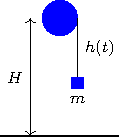
\includegraphics{January2019/1-1.pdf}
\end{center}

}

\sol{}


\prob{1.2}{

A block of mass $M$ slides along a plane surface.
The block is connected to the wall with a spring having spring constant $k$.
A cylinder of mass $m$, radius $R$, and moment of inertia $\frac{1}{2} m R^2$ rolls without slipping on the block.

\begin{parts}

\item What is the frequency of small oscillations of the system around the starting position?

\item Describe the motion associated with the oscillation.

\item What is the maximum oscillation amplitude that the block can have, before the cylinder starts slipping, if the coefficient of static friction between the block and the surface is $\mu$?
    
\end{parts}

\begin{center}
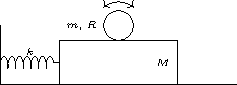
\includegraphics{January2019/1-2.pdf}
\end{center}

}

\sol{}


\prob{1.3}{

A uniform sphere of radius $\rho$ and mass $m$ is constrained to roll without slipping on a lower half of the inner surface of the hollow, stationary cylinder of inner radius $R$ as shown in the figure below, where $g$ is an acceleration of gravity.

\begin{parts}

\item Find the Lagrangian of this system.

\item Find the equation of motion for $\theta(t)$ in the small angle approximation $\sin{\theta} \approx \theta$ and $\cos{\theta} \approx 1 - \theta^2 / 2$.
    
\end{parts}

\begin{center}
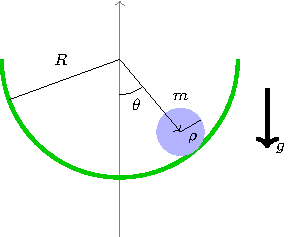
\includegraphics{January2019/1-3.pdf}
\end{center}

}

\sol{}


\prob{1.4}{

Evaluate approximately the ratio of the mass of the earth to the mass of the sun using only the length of the year (365.24 days) and of the lunar month (27.3 days) and the mean radius of the earth's orbit ($1.49 \times 10^8$ km) and of the moon's orbit ($3.8 \times 10^5$ km).

}

\sol{}


\prob{2.1}{

A simple pendulum (mass $M$ and length $\ell$) is suspended from a cart (mass $m$) that oscillates at the end of a spring with a spring constant $k$.

\begin{center}
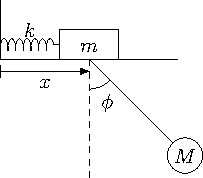
\includegraphics{January2019/2-1.pdf}
\end{center}

\begin{parts}

\item Write down the system's Lagrangian in terms of the variables $x(t)$, $\phi(t)$ and their time-derivatives.

\item Apply the small angle approximation $\sin{\phi} \approx \phi$ and $\cos{\phi} \approx 1 - \phi^2/2$, and show that the Lagrangian can be written in the form
\begin{align}
    L = \frac{1}{2} \dot{X}^{\rm T} M \dot{X} - \frac{1}{2} X^{\rm T} K X
\end{align}
with
\begin{align}
    X = \begin{pmatrix}
        x(t) \\ \phi(t)
    \end{pmatrix}
.\end{align}
Write out the $2 \times 2$ matrices $M$ and $K$ explicitly.

\item Assume that $m = M = \ell = g = 1$ and $k = 2$ (all in appropriate units).
Find the normal frequencies of oscillation.

\item Determine the corresponding normal modes.

\end{parts}

}

%%%%%%%%%%%%%%%%%%%%%%%%%%%%%%%%%%%%%%%%%%
\subsection*{Electricity \& Magnetism} %%%
%%%%%%%%%%%%%%%%%%%%%%%%%%%%%%%%%%%%%%%%%%
\addcontentsline{toc}{subsection}{Electricity \& Magnetism}

\prob{2.2}{

A thin metallic disk of radius $R$ is rotating around its center with the angular frequency $\omega$.
A magnetic induction $B$ is applied along the $z$ axis perpendicular to the disk, as shown in the figure below.

\begin{center}
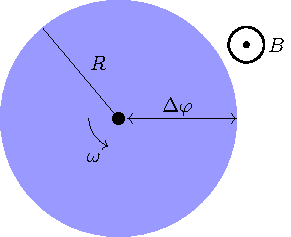
\includegraphics{January2019/2-2.pdf}
\end{center}

\begin{parts}
    \item Calculate the inductive voltage $\Delta \varphi$ between the center of the disk and its edge.
\end{parts}

}

\sol{}


\prob{2.3}{

In a certain inertial frame $S$, at a particular space-time point, the electric field $\vb*{E}$ and the magnetic field $\vb*{B}$ (both non-vanishing) are oriented at an angle $\theta$ to each other ($0 < \theta \leq \pi / 2$).
Consider a different inertial system $S'$, moving relative to $S$ with velocity $\vb*{v}$ in the direction of the electric field $\vb*{E}$.

\begin{parts}

\item Find fields $\vb*{E}'$ and $\vb*{B}'$ at that point in system $S'$.

\item Use your expressions for $\vb*{E}'$ and $\vb*{B}'$ obtained in (a) to explicitly check that
\begin{align}
    \vb*{E}' \cdot \vb*{B}' = \vb*{E} \cdot \vb*{B}
\end{align}
and
\begin{align}
    \vb*{B}'^2 - \vb*{E}'^2 = \vb*{B}^2 - \vb*{E}^2
.\end{align}

\item Show that the angle $\theta'$ between $\vb*{E}'$ and $\vb*{B}'$ is always larger than the angle $\theta$.

\item Is there a frame boosted along $\vb*{E}$ in which $\vb*{E}'$ and $\vb*{B}'$ are \textit{perpendicular}?

\item Is there a frame boosted along $\vb*{E}$ in which $\vb*{E}'$ and $\vb*{B}'$ are \textit{parallel}?
    
\end{parts}

\textbf{Hint}: Transformation of fields for a boost along the $1^{\rm st}$ axis is given by
\begin{align}
    \begin{cases}
        E_1' = E_1 & B_1' = B_1 \\
        E_2' = \gamma(E_2 - \beta B_3) & B_2' = \gamma(B_2 + \beta E_3) \\
        E_3' = \gamma(E_3 + \beta B_2) & B_3' = \gamma(B_3 - \beta E_2)
    ,\end{cases}
\end{align}
where $\beta = v / c$.

}

\sol{}


\prob{2.4}{

Consider a hollow, grounded, conducting sphere of radius $a$.
A point charge $q$ is located at a distance $\rho < a$ from the center of the sphere.
Using the method of images, find:
\begin{parts}

\item the potential $V(r,\theta)$ inside the sphere, where the angle $\theta$ is measured from the axis from the center of the sphere to the charge $q$.

\item the induced charge density on the sphere.
    
\end{parts}

}

\sol{}


\prob{3.1}{

A wire loop of radius $a$ and resistance $R$ lies in the $xy$-plane.
There is a uniform magnetic field $\vb*{B} = B \vu*{z}$ filling the whole space.
What total charge passes a given point in the loop when it is rotated by $90^{\circ}$ around the $x$-axis?

}

\sol{}


\prob{3.2}{

An otherwise free non-relativistic charged particle having mass $m$ and charge $e$ moves in a uniform magnetic field $\vb*{B}$ pointing in the $z$ direction.

\begin{parts}

\item Assume that at $t = 0$ the particle is located at the origin and moving with velocity $\vb*{v}_0$ in the $x$-direction: $vb*{v}_0 = v_0 \vu*{x}$.
Determine the particle's subsequent position $\vb*{r}(t)$ and velocity $\vb*{v}(t)$ as a function of time and describe the resulting motion (ignoring radiation damping).

\item If the initial velocity $\vb*{v}_0$ has both an $x$- and $z$-component, $\vb*{v}_0 = v_0 \vu*{x} + v_0 \vu*{z}$, find the subsequent position $\vb*{r}(t)$ and velocity $\vb*{v}(t)$ as a function of time and describe the resulting motion.
    
\end{parts}

}

\sol{}


\prob{3.3}{

A $\pi^0$ meson with total energy $395~{\rm MeV}$ (in the lab frame) decays into two photons in a symmetric way such that the energies of two photons are equal.
Find the angle between the directions of the momentum vectors of the two photons.

Relevant information: a $\pi^0$ meson is an electrically neutral particle which can decay into two photons.
The rest mass of $\pi^0$ meson is $Mc^2 = 135~{\rm MeV}$.

}

%%%%%%%%%%%%%%%%%%%%%%%%%%%%%%%%%%%
\subsection*{Quantum Mechanics} %%%
%%%%%%%%%%%%%%%%%%%%%%%%%%%%%%%%%%%
\addcontentsline{toc}{subsection}{Quantum Mechanics}


\prob{3.4}{

A particle of mass $M$ moves in one-dimension under the influence of the potential barrier
\begin{align}
    U(x) = \alpha \Big[ \delta(x) - \delta(x - a) \Big]
.\end{align}
Assuming that the incoming wave function at $x < 0$ has the form $e^{ikx}$ with $k > 0$.

\begin{center}
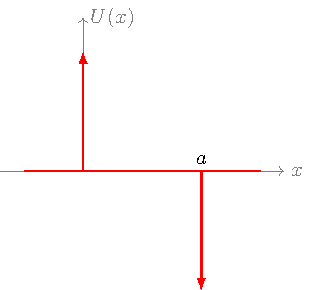
\includegraphics{January2019/3-4.pdf}
\end{center}

\begin{parts}

\item Find energy values $E_n$ for which this particle has zero reflection amplitude (incident from $x < 0$).

\item For the zero reflection energies, find the form of the wave function in the $0 < x < a$ and $x > a$ regions.

\end{parts}

}

\sol{}


\prob{4.1}{

The Hamiltonian of a spin-1 system is given by
\begin{align}
    H = a s_z^2 + b ( s_x^2 - s_y^2 ) + h s_z
,\end{align}
where $a$, $b$, and $h$ are real constants.

Calculate the energy levels using the spin-1 operators:
\begin{align}
    s_x = \frac{1}{\sqrt{2}} \begin{pmatrix}
        0 & 1 & 0 \\ 1 & 0 & 1 \\ 0 & 1 & 0
    \end{pmatrix}
%
,\quad
%
s_x = \frac{1}{\sqrt{2}} \begin{pmatrix}
        0 & -i & 0 \\ i & 0 & -i \\ 0 & i & 0
    \end{pmatrix}
%
,\quad
%
s_z = \begin{pmatrix}
    1 & 0 & 0 \\ 0 & 0 & 0 \\ 0 & 0 & -1
\end{pmatrix}
.\end{align}


}

\sol{}


\prob{4.2}{

Particles with angular momentum 1 are passed through a Stern-Gerlach apparatus which separates them according to the $z$-component of their angular momentum.
Only the $m_z = 1$ component is allowed to pass through the apparatus (with the $z$-axis perpendicular to the beam as it exits the apparatus).
A second apparatus separates the beam according to its angular momentum component along the $u$-axis.
The $u$-axis and the $z$-axis are both perpendicular to the beam direction but have an angle $\theta$ between them.
Find the relative intensities of the three beams separated in the second apparatus.

\textbf{Hint}: This problem can be solved by at least two methods.
\begin{enumerate}

\item Find the eigenstates of $\vb*{\sigma} \cdot \vu*{u}$ in the original coordinate system.
Project the $m_z = 1$ state onto these eigenstates.

\item Apply a rotation around the beam axis of $-\theta$ to the state $m_z = -1$.
This is equivalent to rotating the coordinate system by $\theta$.
The resulting states $(1,0,0)$, $(0,1,0)$, and $(0,0,1)$ are now eigenstates of $\vb*{\sigma} \cdot \vu*{u}$

\end{enumerate}

}

\sol{}


\prob{4.3}{

Write the Sch\"{o}dinger equation for a 1-dimensional harmonic oscillator in the momentum representation.

Determine the probability density for the lowest momentum state.

}

\sol{}


\prob{4.4}{

For the infinite square well with walls located at $x = a$ and $x - -a$, the ground state energy is $E_1 = \pi^2 \hbar^2 / (8 m a^2)$ and the ground state wavefunction is $\psi_1(x) = \frac{1}{\sqrt{a}} \cos(\pi x / 2a)$.
The position-momentum uncertainty relationship for this state is $\Delta x \Delta p = k \hbar / 2$.
Find $k$.

A potentially useful formula is
\begin{align}
    \int \dd{x} x^2 \cos^2(bx) = \frac{x^3}{6} + \Big( \frac{x^2}{4 b} - \frac{1}{b^3} \Big) \sin(2 b x) + \frac{x \cos(2 b x)}{4 b^2}
\end{align}

}
